\documentclass[letterpaper, 12pt]{article}
\usepackage{graphicx}
\graphicspath{{Figures/}{./}}
\usepackage{apacite}
\usepackage{amsmath}
\usepackage{amssymb}
\usepackage{amsthm}
\usepackage{indentfirst}
\usepackage[justification=centering]{caption}
\usepackage{float}

\title{MATHEMATICS ANALYSIS AND APPROACHES HL
\\
Producing the IB Logo with the Fourier Series}
\author{}
\date{}

\begin{document}
\nocite{*}

\maketitle
\begin{center}
    Candidate Code:
    \\
    Session: May 2024
    \\
    Page Count:
\end{center}
\newpage

\tableofcontents
\newpage

\section{Rationale}

I have shown interest in visual arts done through the means of software,
with particular experience in 3D modelling and animation in Blender
and Cinema 4D.

I never was experienced with drawing, therefore producing digital art
on a 2D plane using artistic skill was not of interest to me. However,
something that I came across online was the use of the Fourier Series
in order to produce vector art, which instantly intrigued me.

While vector art files such as those with the file extension ".svg" relate
to mathematics in the sense that it contains multiple graphed mathematical
relationships in order to produce an image, the method of using the Fourier
Series to produce similar art is more mathematically intriguing, as it
proves use just one expression to produce the same result done by the numerous mathematical
relationships.


\section{Aim}

The objective of this investigation is to link Fourier series with
complex numbers to create a single series that is capable
of reproducing the IB logo on the Argand plane.

\section{Plan of Action}

This exploration focuses on the following areas of math:
\begin{itemize}
    \item Integral Calculus
    \item Series
    \item Trigonometry
    \item Complex Analysis
    \item Vectors
\end{itemize}

\section{Background Information}

\subsection{Overarching idea of the Fourier Series}

A periodic function is one where the output for a particular input equals to
the output for the sum of the same input and the value of the function's period.
This can be represented mathematically as:
\begin{align*}
     & f(x) = f(x + P)
    \\
     & \text{where } P = \text{ the period of the function}
\end{align*}

The sine wave is widely known for being a periodic function for the ease of graphing
a sinusoidal wave. However, there are periodic functions that are difficult to
graph with an algebraic expression, such as one that alternates between
1 and -1 or one that is shaped as a zig-zag.

This is the motivation behind the Fourier Series, which is to be able to represent
period functions that normally can't be represented by an algebraic function.

The idea behind the Fourier Series is to take an infinite sum of varying sinusoidal
functions such that a desired periodic function is produced.

\begin{figure}[H]
    \centering
    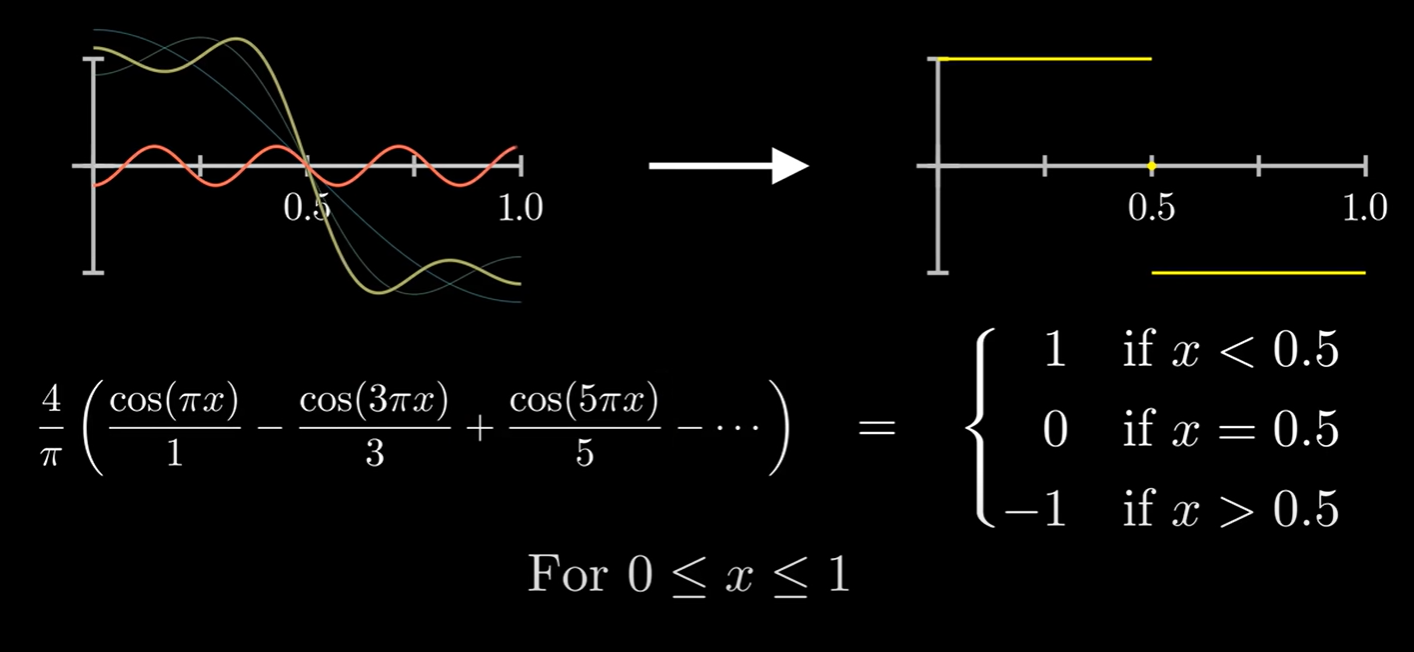
\includegraphics[width=\textwidth]{fourier_basic_visual.png}
    \caption{Visualization of the mechanism of the Fourier Series \protect\cite{sandersonWhatFourierSeries2019}. The yellow line is the periodic function resulting from the previous iteration, the red line is the sinusoidal function to be added in the next iteration.}
    \label{fig:fourier_visual}
\end{figure}

% For reference, a general formula for representing a periodic function as a Fourier Series with a
% period of \(2\pi\) is:
% \begin{equation}
%     f(t) = \frac{a_0}{2} + \sum_{n = 1}^{\infty} a_n \cos{nt} + \sum_{n=1}^{\infty} b_n\sin{nt}
% \end{equation}

% This formula won't be explored in depth, however, it is included as it will
% emphasize how the Fourier Series can be linked with complex numbers.

\subsection{Idea of drawing with the Fourier series explained with the Cartesian Plane}

The rule is for eligible drawings to be any that can be drawn by starting at one point
on a cartesian plane and, without lifting the hypothetical plane throughout the entire
sketch, return to the exact same point.

Defining the variable \(t\) as time, \(t = 0\) will represent the point in time
where the drawing began and \(t = 1\) will represent the point in time where
the drawing ended.

Each point of the drawing on the plane will be defined by \(P(x(t), y(t))\),
where \(x(t)\) and \(y(t)\) are both functions with an input of \(t\) that
indicates the coordinates after some amount of time passed of the pen's progress
through the drawing.

Assuming that any function can be represented as a Fourier Series, then
\(x(t)\) and \(y(t)\) can be any function and therefore, by extracting
the coordinates on a graph of any drawing obeying the rule described earlier,
the Fourier Series of \(x(t)\) and \(y(t)\) can be determined and therefore
produce the desired drawing for \(t\in [0,1]\)
\\

As a simple example that does not require a Fourier Series,
we can take a unit circle defined by \( x^2 + y^2 = 1 \) as the drawing.
It quickly becomes evident of what \(x(t)\) and \(y(t)\) are, as since it is a circle,
then \(x(t) = \cos(2\pi t)\) and \(y(t) = \sin(2\pi t)\).

\subsection{Enriched application to draw on the Argand Plane} \label{sec:big_guy}

Euler's formula is defined to be
\begin{equation}
    e^{it} = \cos(t) + i\sin(t)
    \label{eq:euler}
\end{equation}

Given that both the cosine function and the sine function are included in this
formula, a connection between this formula and the Fourier Series becomes evident.
The two sinusoidal functions in the formula are the core behind applying the
Fourier Series to the Argand Plane.

It is easier to think of Euler's formula to be a vector on the Argand Plane \cite{sandersonWhatFourierSeries2019}.
With just the formula given above, we have a vector with a length of 1 that rotates
counterclockwise when the value that \(e\) is raised to is positive and
clockwise when the value is negative.

Let's incorporate \(n\) and \(2\pi\) to the power in Equation \textbf{(\ref*{eq:euler})} such
that we have \(e^{n \cdot 2\pi it}\). The purpose of \(2\pi\) is to
simplify what defines a revolution, as now, for every unit of time that
\(t\) passes, a revolution will be completed. \(n, n \in \mathbb{Z}\) will define the frequency
and directionality of the rotation of the vector. If \(n > 0\), then the vector
will rotate counterclockwise and vice versa. If \(n = 2\), then the vector would
rotate by 2 revolutions for every unit of time that passes.

Lastly, let's multiply the entire power by the variable \(c_n\) to get \(c_n e^{n \cdot 2\pi it}\). This will not
only allow for the vector to be scaled but also for the starting rotation of
the vector to be defined. Let's temporarily define \(c_n\) to be:

\begin{equation*}
    c_n = A \cdot z
\end{equation*}

\(A\) will indicate the factor to which the vector will be scaled by. Because
the original length of the vector was 1, then the factor will directly indicate
the length of the vector.

\(z\) will indicate the starting rotation of the vector, which would be
\(e^{i\theta}\), where \(\theta\) is the starting rotation angle in radians.
\\

It could be imagined that the final Fourier Series that produces a desired drawing
is the sum of multiple vectors of different magnitudes rotating a different frequencies
indicated by \(n, n \in \mathbb{Z}\). Therefore, if \(f(t)\) is defined to be the
function that represents the drawing, this can be expressed mathematically
as:

\begin{equation}
    f(t) = \sum_{n=-\infty}^{\infty} c_n e^{n \cdot 2\pi it}
    \label{eq:ft_def}
\end{equation}

The main concern as of right now is how the value of \(c_n\) will be determined
for a specific drawing.

The easiest way to start off is by first considering \(c_0 e^{0 \cdot 2\pi it}\).
This can be simplified into \(c_0\), but what does this mean?
This is the vector that is rotating at a frequency of 0, which means that
it is static. It can therefore be defined to be the "centre of mass"\cite{sandersonWhatFourierSeries2019}
of the entire function.

If we take discrete intervals of \(t\) and obtain the value of \(f(t)\),
then by taking the average of all those values, we obtain a complex number
close to \(c_0\). This is illusrated by Figure \ref{fig:cnot_integ}.

\begin{figure}[H]
    \centering
    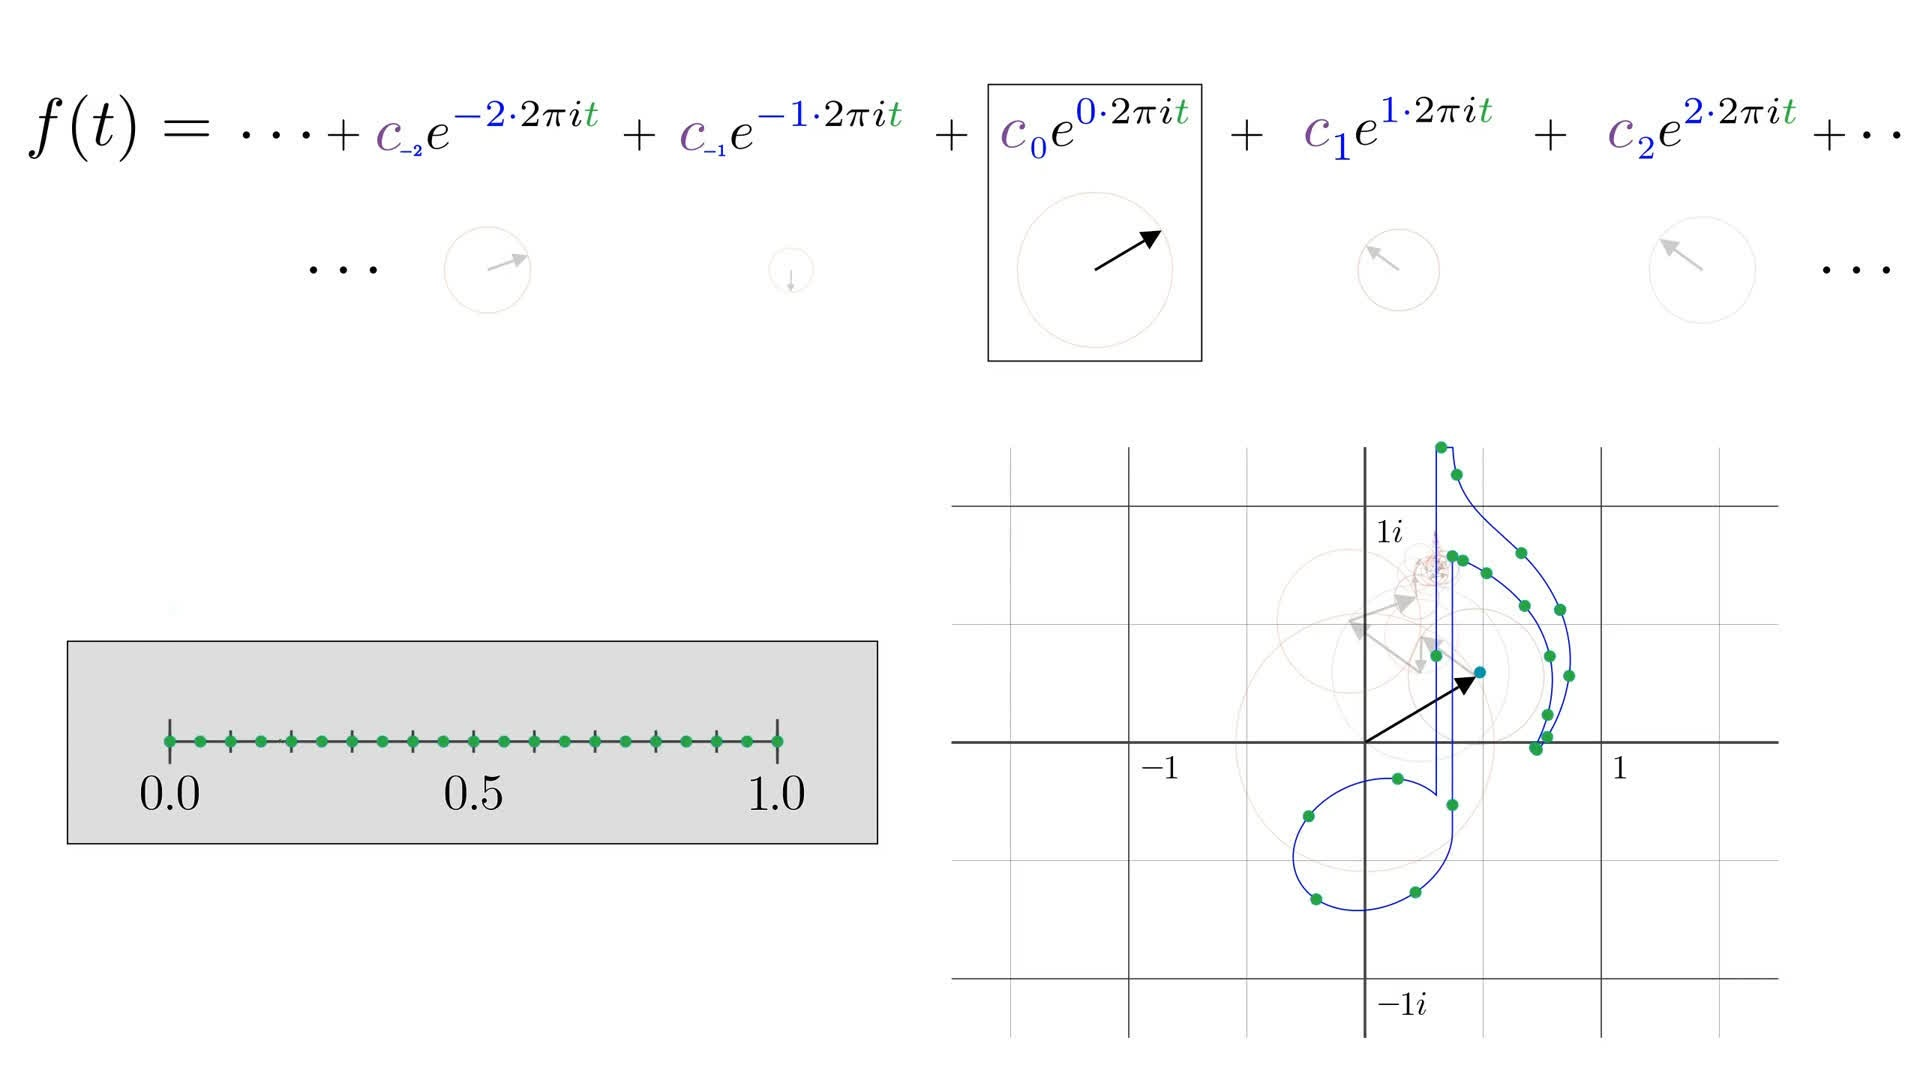
\includegraphics[width=\textwidth]{cnot_integ.jpeg}
    \caption{Averaging points throughout \protect\(f(t)\) illustrated \protect\cite{sandersonWhatFourierSeries2019}. The number line represent \protect\(t\), and the red dots on the musical note represent the resulting values of \protect\(f(t)\)}
    \label{fig:cnot_integ}
\end{figure}

With finer and finer intervals of \(t\), the result
becomes more and more accurate to the value of \(c_0\), therefore it can be
said that:

\begin{equation}
    c_0 = \lim_{\Delta t \to 0} \sum_{t = 0}^{\frac{1}{\Delta t}} f(t \cdot \Delta t) \Delta t
    \label{eq:cnot_lim}
\end{equation}

From Equation \textbf{(\ref*{eq:cnot_lim})}, \(c_0\) can ultimately be expressed as:

\begin{equation}
    c_0 = \int_{0}^{1} f(t) \,dt
    \label{eq:cnot_integ}
\end{equation}


We can use the same technique for all other values of \(n\), but the problem is
for all other values of \(n\) that are not 0, the vector is rotating, therefore
it doesn't make sense to take the average of the rotating vector.

Recalling the thorough definition of \(f(t)\) stated earlier in Equation \ref*{eq:ft_def},
we can substitute Equation \ref*{eq:ft_def} into Equation \ref*{eq:cnot_integ}.

\begin{align*}
     & c_0 = \int_{0}^{1} \sum_{n=-\infty}^{\infty} c_n e^{n \cdot 2\pi it} \,dt
    \\
     & c_0 = \int_{0}^{1} \left( \cdots + c_{-1} e^{-1 \cdot 2\pi it} + c_{0} e^{0 \cdot 2\pi it} + c_{1} e^{1 \cdot 2\pi it} + \cdots \right) \,dt
    \\
     & c_0 = \cdots + \int_{0}^{1} c_{-1} e^{-1 \cdot 2\pi it} \,dt + \int_{0}^{1} c_{0} e^{0 \cdot 2\pi it} \,dt + \int_{0}^{1} c_{1} e^{1 \cdot 2\pi it} \,dt + \cdots
\end{align*}

Remember that \(\int_{0}^{1} c_{0} e^{0 \cdot 2\pi it} \,dt\) was easy to simplify
as the power cancels out from being raised to 0. In turn, it can be further
evaluated to be just \(c_0\), as shown below:

\begin{align*}
     & \int_{0}^{1} c_{0} e^{0 \cdot 2\pi it} \,dt
    \\
     & = \int_{0}^{1} c_{0} \,dt
    \\
     & = [c_{0}t]_{0}^1
    \\
     & = c_{0}
\end{align*}

Additionally, if all the other integrals were thought of as the the average of all
the points produced when its vector rotates by one revolution, then it can
be argued that each integral, when evaluated, would be 0.

This idea is illustrated in Figure \ref*{fig:circle_integ}.

\begin{figure}[H]
    \centering
    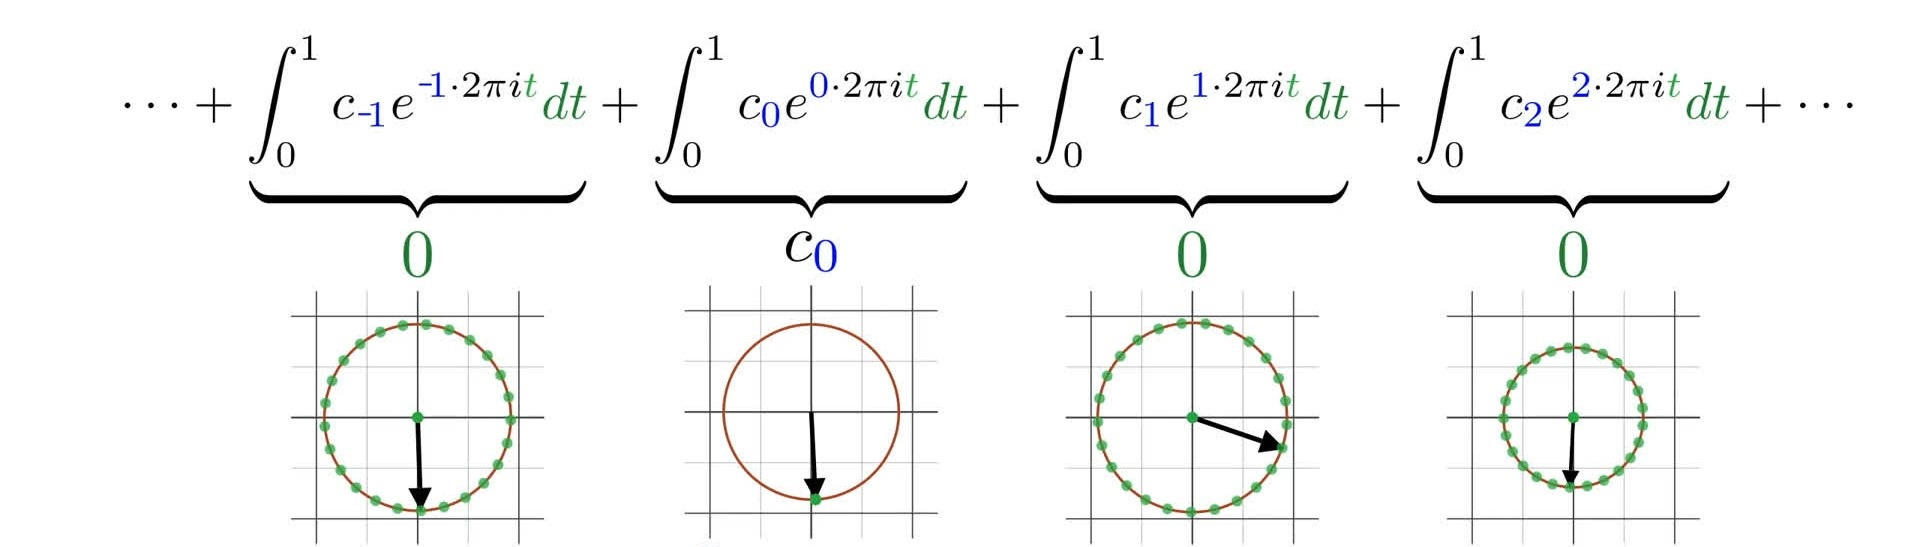
\includegraphics[width=\textwidth]{circle_integ.jpeg}
    \caption{Illustration of averaging all the points on a circle \protect\cite{sandersonWhatFourierSeries2019}.}
    \label{fig:circle_integ}
\end{figure}

If we were to multiply \(f(t)\) by \(e^{-n \cdot 2\pi it}\), then an effect can occur
where all of the power's exponents will decrease by \(n\). Ultimately, we will
get a similar scenario in the summation of all the integrals where
all integrals are evaluated to become 0 except for the integral
where \(n = 0\), which evaluates to \(c_0\). However, the multiplication
of the two powers will cause the integral of some \(n\) value to simplify to just
\(c_n\).

This mechanism is mathematically shown below.
\begin{align*}
     & n = 1
    \\
     & c_1 = \int_{0}^{1} f(t) e^{-1 \cdot 2\pi it} \,dt
    \\
     & c_1 = \cdots + \int_{0}^{1} c_{-1} e^{-1 \cdot 2\pi it} \cdot e^{-1 \cdot 2\pi it} \,dt
    \\
     & + \int_{0}^{1} c_{0} e^{0 \cdot 2\pi it} \cdot e^{-1 \cdot 2\pi it} \,dt + \int_{0}^{1} c_{1} e^{1 \cdot 2\pi it} \cdot e^{-1 \cdot 2\pi it} \,dt + \cdots
    \\
     & c_1 = \cdots + \int_{0}^{1} c_{-1} e^{-2 \cdot 2\pi it} \,dt + \int_{0}^{1} c_{0} e^{-1 \cdot 2\pi it} \,dt + \int_{0}^{1} c_{1} e^{0 \cdot 2\pi it} \,dt + \cdots
    \\
     & c_1 = \cdots + 0 + 0 + c_1 + 0 + 0 + \cdots
    \\
     & c_1 = c_1
\end{align*}

Therefore, \(c_n\) can be defined as:

\begin{equation}
    c_n = \int_{0}^{1} f(t) e^{-n \cdot 2\pi it} \,dt
    \label{eq:cn_integ}
\end{equation}

Equation \ref*{eq:cn_integ} is what will be used in order to
determine each value of \(c_n\)
\\

All concepts of this section come from \cite{sandersonWhatFourierSeries2019}.


\subsection{Bezier Curves}


\subsection{Composition of ".svg" files}


\subsection{Contour integration?}
(This is just a placeholder. This concept may enrich this IA, although
I do not yet know enough to foresee if understanding this concept
will be something that is achievable)




\section{Methodology}

\subsection{Analysis of ".svg" Files}

\subsection{Computation of parameters}

Given that \(f(t)\) is able to be determined as a piecewise function
from the previous section, the desired summation representing
\(f(t)\) can be determined.

Referring back to Section \ref*{sec:big_guy}, \(c_n\) is defined as:

\begin{equation*}
    c_n = \int_{0}^{1} f(t) e^{-n \cdot 2\pi it} \,dt
\end{equation*}

This means that every \(c_n\) must be determined individually. Therefore,
it becomes evident that it is unreasonable to evaluate the infinite sum of
\(f(t) = \sum_{n=-\infty}^{\infty} c_n e^{n \cdot 2\pi it}\), and that
the limits of the summation must be defined.

Let's rewrite \(f(t)\) as:
\begin{equation*}
    f(t) = \sum_{n=-k}^{k} c_n e^{n \cdot 2\pi it}
\end{equation*}

so that \(k\) indicates the frequency of the two fastest vectors
that are spinning in opposite directions to each other.

As \(k \to \infty\), \(f(t)\) becomes more and more accurate to
the original drawing, which will be demonstrated by performing distinct
analyses for various values of \(k\).

\subsubsection{Approach 1: Numerical Integration}

\begin{equation*}
    c_n = \int_{0}^{1} f(t) e^{-n \cdot 2\pi it} \,dt
\end{equation*}

The integral above can be evaluated for some value of \(n\) by
taking some small value to represent \(\Delta t\), in which
by summing up the values from \(f(t) e^{-n \cdot 2\pi it}\)
produced by each increment of \(t\) by \(\Delta t\), a value close
to the original integral can be determined \cite{sandersonWhatFourierSeries2019}.

\begin{equation}
    c_n = \sum_{t = 0}^{\frac{1}{\Delta t}} f(t \cdot \Delta t) e^{-n \cdot 2\pi i(t \cdot \Delta t)} \Delta t
\end{equation}

\subsection{Rendering the final image}

\bibliographystyle{apacite}
\bibliography{IB_MATH_IA.bib}

\end{document}